\section{Aufgabe1}
\label{sec:Aufgabe1}
\paragraph{Wiederholung der Methoden aus der Vorlesung}
Gegeben:
\begin{equation}
 f(u) = U(0,1) = 
\begin{cases}
1, & 0 \leq x < 1 \\
0, & \text{sonst}
\end{cases}	
\end{equation}
Hier bezeichnet u gleichverteilte Zufallsvariablen mit der Wahrscheinlichkeitsdichte $f(u)$. 
Gesucht: 
\begin{equation}
g(y) \quad \text{mit} \quad y \in [y_{min},y_{max}]	
\end{equation}
Dabei bezeichnet $y$ eine Zufallsvariable mit der Wahrscheinlichkeitsdichte $g(y)$. 
Die Transformation einer Gleichverteilung, um Zufallszahlen aus einer beliebigen Verteilung 
zu generieren ist gegeben durch
\begin{gather}
g(y) \symup{d} = U(0,1)\symup{du} \\
\implies u = \int_{u_{min}} ^{u} U(0,1) \symup{d}u  = G(y) = \int_{y{min}} ^{y} g(y') \symup{d}y' \\
\implies y = G^{-1}(u) \; .
\label{eq:methods}
\end{gather}
Für den Programmierteil dieser Aufgabe wurden die zufälligen Werte wie folgt erstellt.
\lstinputlisting[language=Python, firstline=16, lastline=18]{plots/Aufgabe1.py} 


\subsection{a)}
Mit den zuvor dargestellten Methoden ergibt sich die Funktion
\begin{equation}
y = u \cdot (b-a) + a \; .
\end{equation}
Die dazugehörigen Rechnungen sind in der Abbildung \ref{fig:A1ab} dargestellt.
In der Abbildung \ref{fig:A1abcd} in der oberen linken Ecke findet sich ein Histogramm der 
Funktion (grün). Im selben Histogramm ist die gegebene Gleichverteilung die Werte in 
den Grenzen [0,1] ausgibt gezeigt. In Python wurde die Funktion wie folgt implementiert.

\lstinputlisting[language=Python, firstline=20, lastline=21]{plots/Aufgabe1.py}

\subsection{b)}
Mit den zuvor dargestellten Methoden ergibt sich die Funktion
\begin{equation}
y = - \tau \ln(1-u) \; .	
\end{equation}
Die dazugehörigen Rechnungen sind in der Abbildung \ref{fig:A1ab} dargestellt.
In der Abbildung \ref{fig:A1abcd} in der oberen rechten Ecke findet sich ein Histogramm der 
Funktion (blau).In Python wurde die Funktion wie folgt implementiert.

\lstinputlisting[language=Python, firstline=23, lastline=24]{plots/Aufgabe1.py}


\subsection{c)}
Mit den zuvor dargestellten Methoden ergibt sich die Funktion
\begin{equation}
y = \left( u \cdot \left(b^{1-n} - a^{1-n} \right) + a^{1-n} \right)^{\frac{1}{1-n}} \; .
\end{equation}
Die dazugehörigen Rechnungen sind in der Abbildung \ref{fig:A1cd} dargestellt.
In der Abbildung \ref{fig:A1abcd} in der unteren linken Ecke findet sich ein Histogramm der 
Funktion (blau).In Python wurde die Funktion wie folgt implementiert.

\lstinputlisting[language=Python, firstline=26, lastline=27]{plots/Aufgabe1.py}

\subsection{d)}
Mit den zuvor dargestellten Methoden ergibt sich die Funktion
\begin{equation}
y = \tan ( \pi (u +1 ))
\end{equation}
Die dazugehörigen Rechnungen sind in der Abbildung \ref{fig:A1cd} dargestellt.
In der Abbildung \ref{fig:A1abcd} in der unteren rechten Ecke findet sich ein Histogramm der 
Funktion (blau).In Python wurde die Funktion wie folgt implementiert.

\lstinputlisting[language=Python, firstline=29, lastline=30]{plots/Aufgabe1.py}

\begin{figure}
\begin{subfigure}{.48\textwidth}
  \centering
  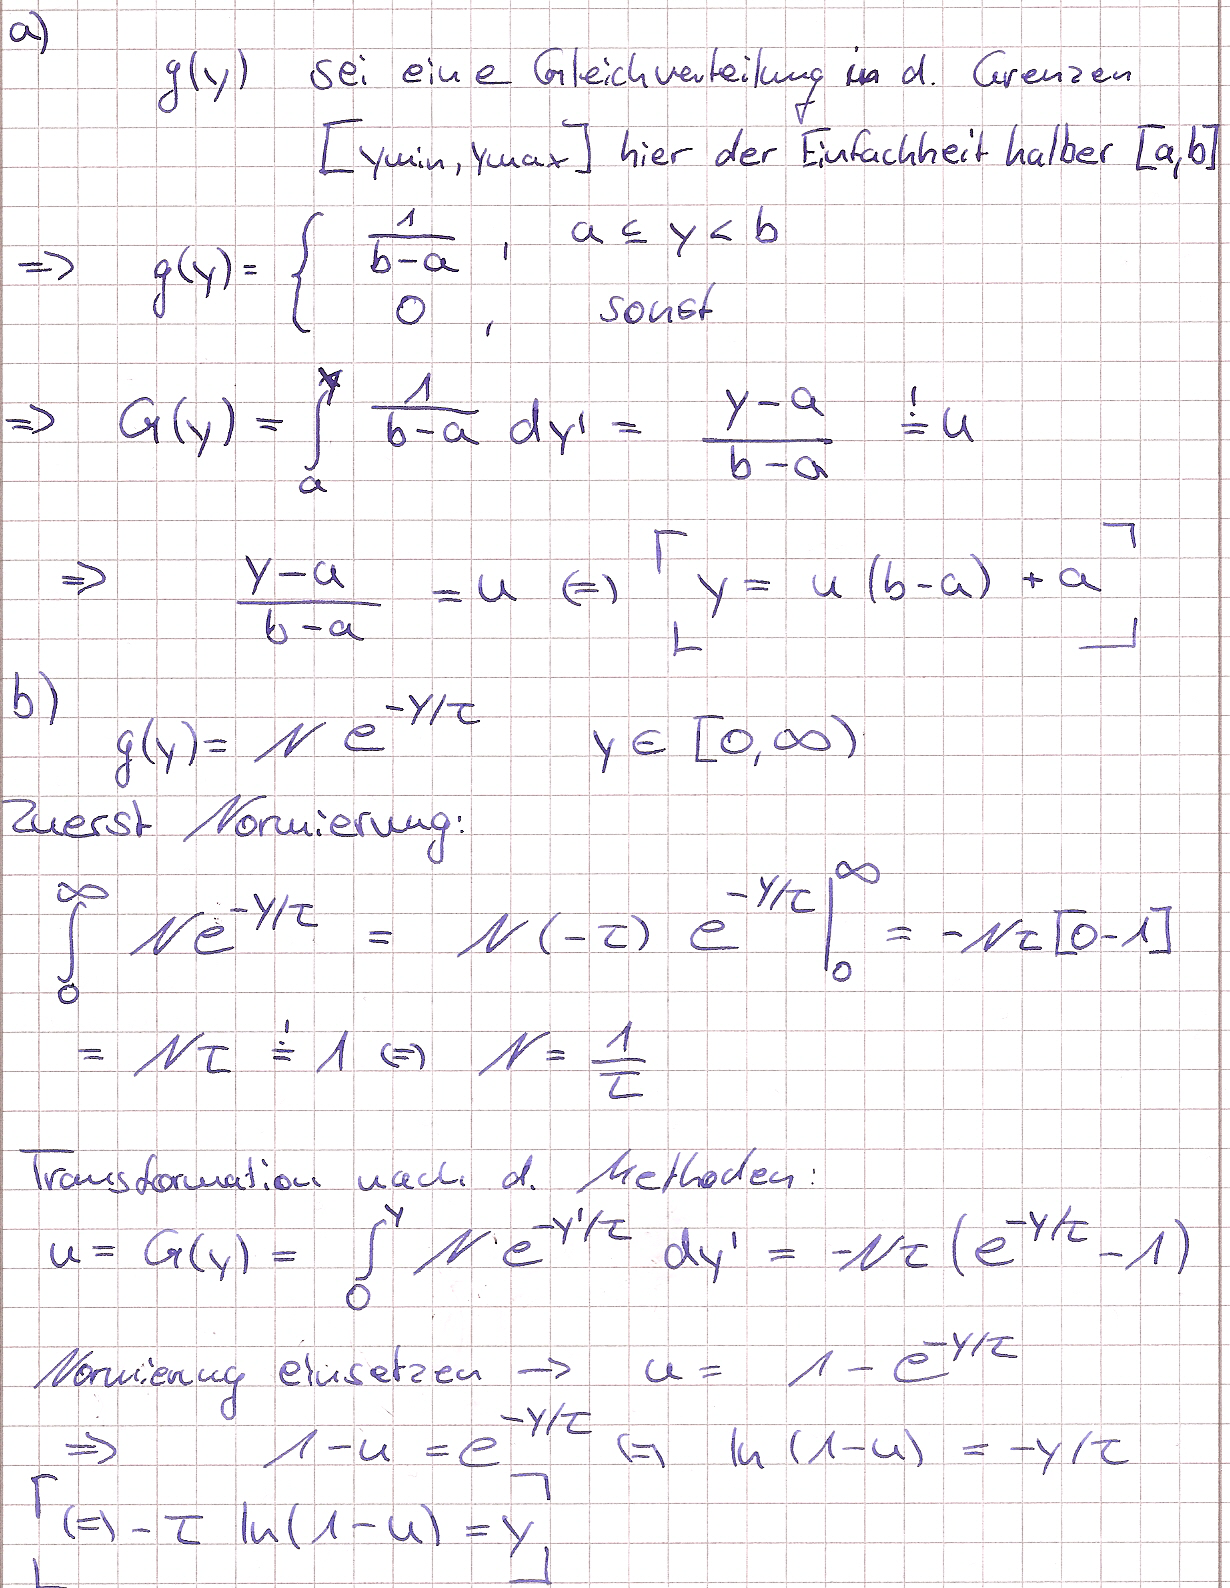
\includegraphics[height = 10cm]{pics/A1ab}
  \caption{a) und b).}
  \label{fig:A1ab}
\end{subfigure}
\begin{subfigure}{.48\textwidth}
  \centering
  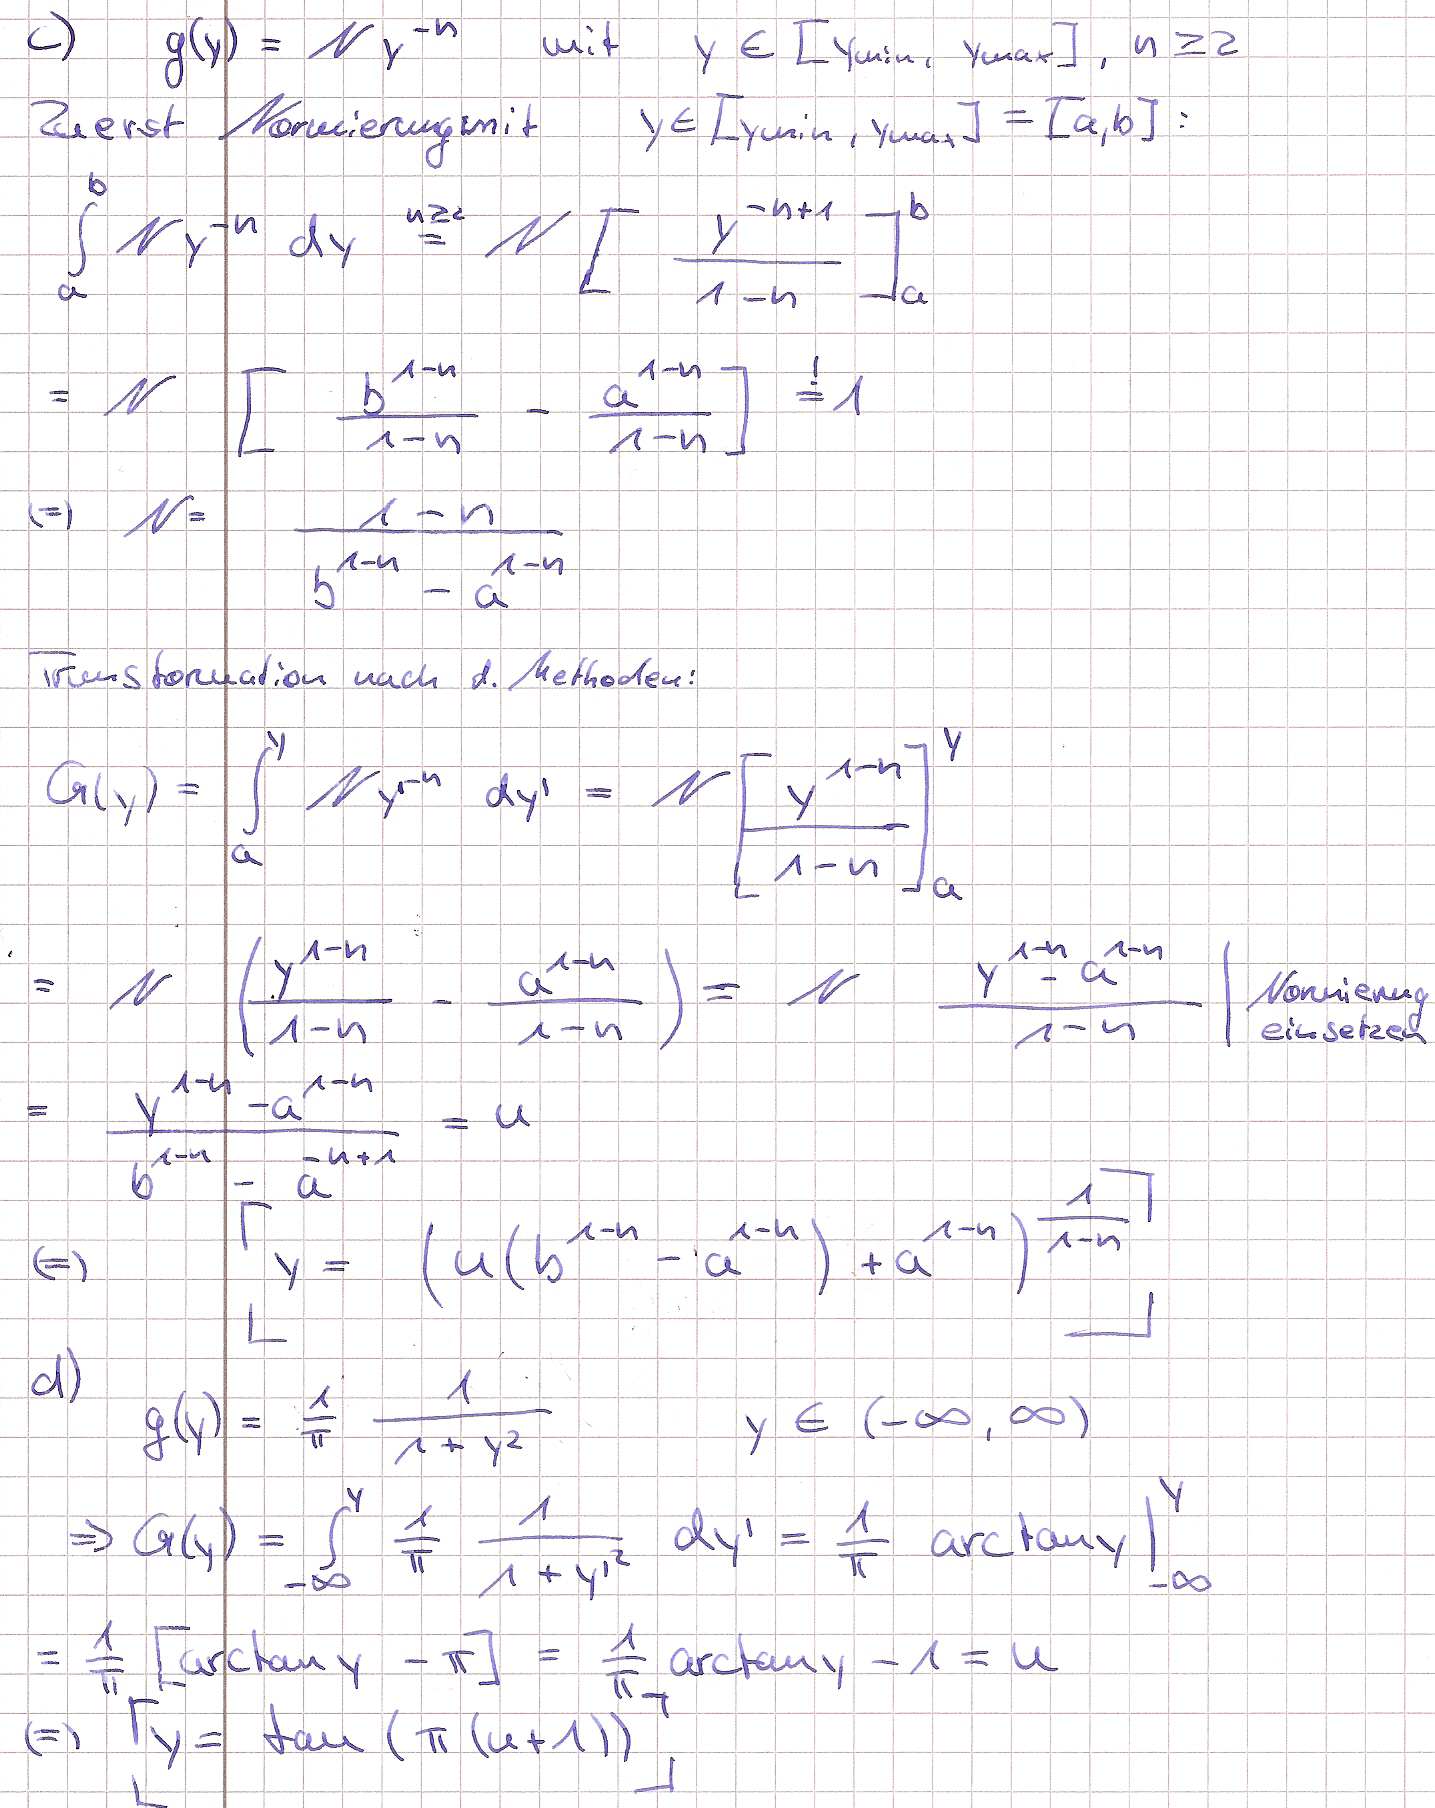
\includegraphics[height = 10cm]{pics/A1cd}
  \caption{c) und d).}
  \label{fig:A1cd}
\end{subfigure}
  \caption{Rechnungen zu Aufgabe1}
  \label{fig:A1rech}
\end{figure}

\begin{figure}
  \centering
  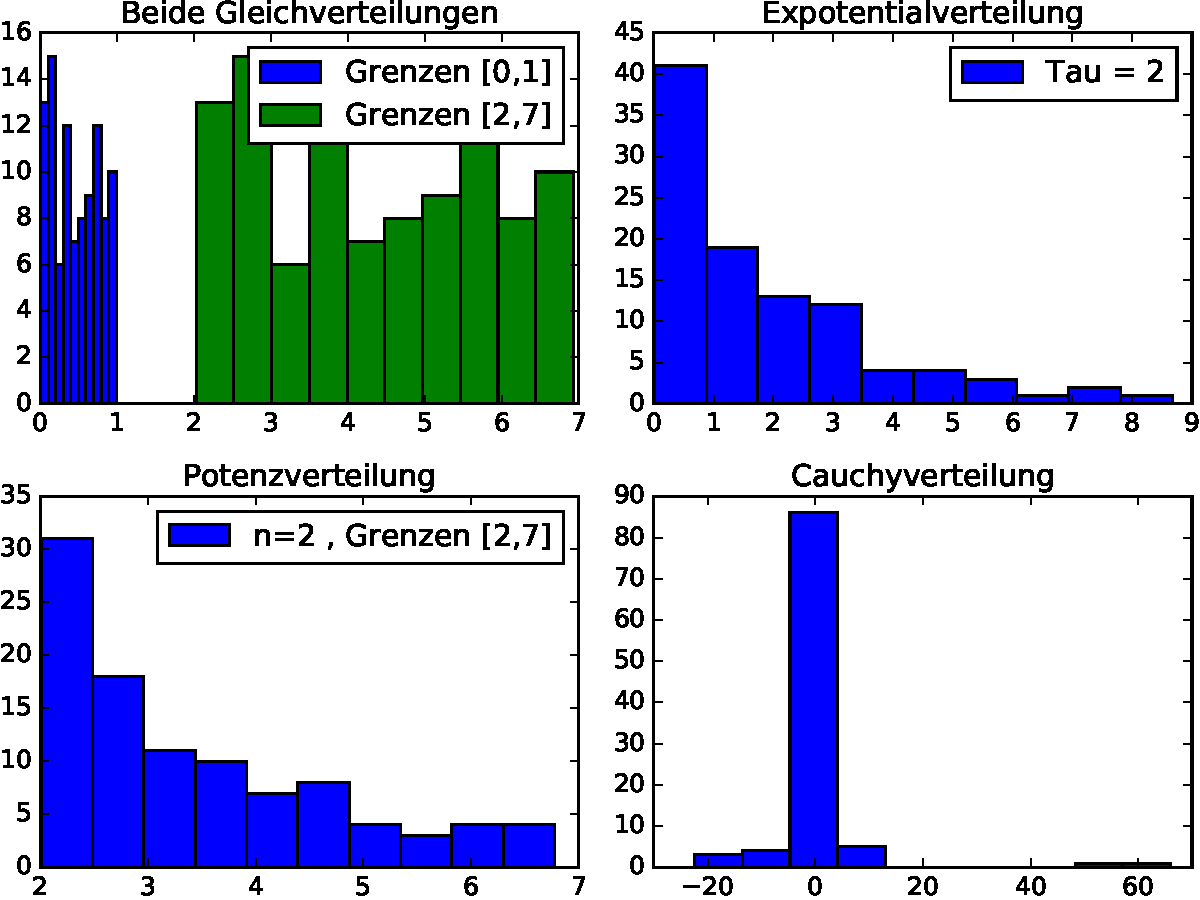
\includegraphics[height = 10cm]{plots/A1abcd.pdf}
  \caption{Diagramme zu den einzelnen Verteilungen.}
  \label{fig:A1abcd}
\end{figure}


\subsection{e)}
Eine Methode um aus diskreten Werten Zufallsvariablen zu generieren ist, zuerst eine 
kummulative Wahrscheinlichkeit für alle $x_k$ mit $k = 1, ... ,n$ zu berechnen, mit 
\begin{equation}
P_{k+1} = \sum_{i=1} ^{k} P(x_i) \quad \text{mit} \quad P_1 = 0 , \; P_{n+1} = 1 \; .
\end{equation}
Das wurde von uns in Python wie folgt implimentiert.

\lstinputlisting[language=Python, firstline=32, lastline=39]{plots/Aufgabe1.py}
Hier stellt \textit{wahrsch} die Wahrscheinlichkeit berechnet aus den Counts da und 
\textit{kumuwahr} die kummulative Wahrscheinlichkeit. Die for-Schleife führt eigentlich nur die 
Summe aus. 
Um nun die diskreten Zufallsvariablen zu bekommen nimmt man die gleichverteilten Zufallswerte $u$ 
und vergleicht diese mit den Elementen $P_{k-1} < u < P_k$ so erhält man den Index $k$ für den 
die Ungleichung erfüllt ist. Der Index ist dann auch der Index der diskreten Zufallsvariable 
anhand dem man die Zufallsvarable auslesen kann. In dem Fall hier ist es der Index eines 
\textit{binmid} Wertes. Die Inplementierung in Python folgt.
 
\lstinputlisting[language=Python, firstline=40, lastline=47]{plots/Aufgabe1.py}
Das Historgamm dazu ist in der Abbildung \ref{fig:A1eplot} dargestellt.
\begin{figure}
  \centering
  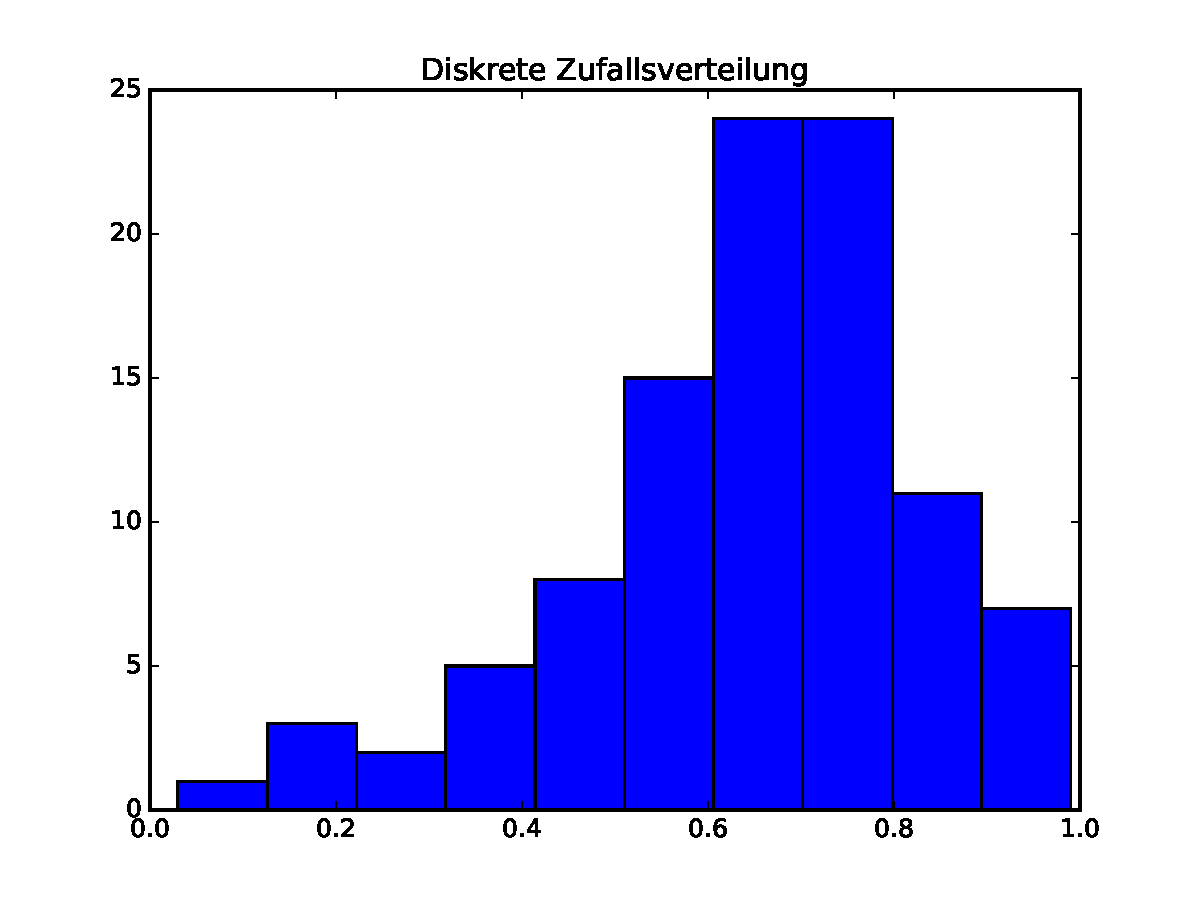
\includegraphics[height = 10cm]{plots/A1eplot.pdf}
  \caption{Histogramm zu den diskreten Zufallsvariablen.}
  \label{fig:A1eplot}
\end{figure}
 

